\chapter{Simulate simple 2D Brownian motion of $\textbf{\textit{E.coli}}$} % Main chapter title

\label{Part1_chapter} % For referencing the chapter elsewhere, use \ref{Chapter1} 

\section{Symbols}

\begin{table}[H]
\caption{The symbols used in the model of simulating simple 2D Brownian motion of $E.coli$ }
\label{tab:part1_symbols}
\centering
\begin{tabular}{l l}
\toprule

\tabhead{Symbol} & \tabhead{Definition} \\
\midrule
$X(t)$ & Stochastic processes \\
$X_i$ & The direction of movement $X_i = 1,\ -1$\\
$B(t)$ & Standard Brownian Motion \\
$N(\mu,\sigma)$ & Normal distribution with mean $\mu$ and standard deviation $\sigma$ \\
% ${\rm R^{2}_{i}}$ 改成正常体
$\Delta x$ & Space interval \\
$\Delta t$ & Time interval \\
$\qquad \sigma  $ & $\qquad \sigma = \Delta x$/$\sqrt{ \Delta t}$ \\
$(x,y)$ & Coordinates of $E.coli$ \\
$\qquad x_t  $ & \qquad Coordinate in x axis at time t \\
$\qquad y_t  $ & \qquad Coordinate in y axis at time t \\
$v$			   & The speed of the movement of $E.coli$ \\
\bottomrule\\
\end{tabular}
\end{table}


\section{Biological background}

$Escherichia \ coli$ is a Gram-negative, optional anaerobic, rod-shaped, coliform bacterium of the genus Escherichia that is commonly found in the lower intestine of warm-blooded organisms. $E.coli$ are widely used in biological research, cells are typically rod-shaped, and are about 2.0 $\mu m$ long and 0.25-1.0 $\mu m$ in diameter, with a cell volume of 0.6-0.7 $\mu m^3$ . Strains that possess flagella are motile. The flagella have a peritrichous arrangement.It also attaches and effaces to the microvilli of the intestines via an adhesion molecule known as intimin. The thin straight filaments of bacteria called pili, that enable it to attach to specify substrate, and thicker longer helical filaments, called flagella, that enable it to swim.

Brownian motion is the random motion of microscopic particles suspended in a fluid resulting from their collision with the quick atoms or molecules in the liquid or gas. This phenomenon is named after British botanist Robert Brown. In 1827, while looking through a microscope at particles trapped in cavities inside pollen grains in water, Brown noted that the particles moved through the water randomly but failed to explain the mechanisms that caused this movement. He supposed that active molecules were inside those particles thus there was no relationship with the surrounded liquid. 

The Brownian motion is a Gaussian process with time $t$, we can find that, for stochastic processes $\{X(t),t\geq0\}$ :

\begin{equation*} 
\begin{aligned} 
\centering
X(0) &= 0 \\
X(t) &\backsim N(0,\sigma^2t)  \\ 
X(t) &= \Delta x(X_1 + ... + X_{[t/\Delta t]}) \\
\sigma^2 &=  \frac{(\Delta x)^2}{\Delta t} \\
\end{aligned} 
\end{equation*}

\newpage
Normally, we set $\sigma=1$ and defines this kind of stochastic processes $\{X(t),t\geq0\}$ as \textbf{Standard Brownian Motion} and they could be denote as $\{B(t),t\geq0\}$, where :

\begin{equation*} 
\begin{aligned} 
\centering
B(0) &= 0 \\
B(t) &\backsim N(0,t)  \\ 
\end{aligned} 
\end{equation*}

\section{Hypothesis for simulation}

Assuming the $E.coli$ here have no mitosis, so the number of cells maintain constant.
I use $(x,y)$ to define the location of each cell, assume all the cells start from origin$(0,0)$. They have a random judging for each step in both x and y directions. Set the speed as $50 \mu m/s$, so for each step,


\begin{equation*} 
\begin{aligned} 
\centering
\phi_x &\backsim N(0,1) \\
\phi_y &\backsim N(0,1) \\
x_{t+1}  &=  x_{t} + \phi_x v \\ 
y_{t+1}  &=  y_{t} + \phi_y v \\ 
\end{aligned} 
\end{equation*}
The move on both x and y directions are random and it follows the Brownian motion.\\
So in theory, for a $E.coli$ population large enough, we have: \\
\begin{equation*} 
\begin{aligned} 
\centering
\frac{1}{n} \sum_{i=1}^{n}x_i(t)   &\approx 0 \\
\frac{1}{n} \sum_{i=1}^{n}y_i(t)   &\approx 0 \\
\frac{1}{n} \sum_{i=1}^{n}x_i(t)^2 &\approx v^2t  = 250t \\
\frac{1}{n} \sum_{i=1}^{n}y_i(t)^2 &\approx v^2t  = 250t \\
\end{aligned} 
\end{equation*}
%----------------------------------------------------------------------------------------
%\newpage
\section{Results of simulation}

\begin{figure}[H]
\centering
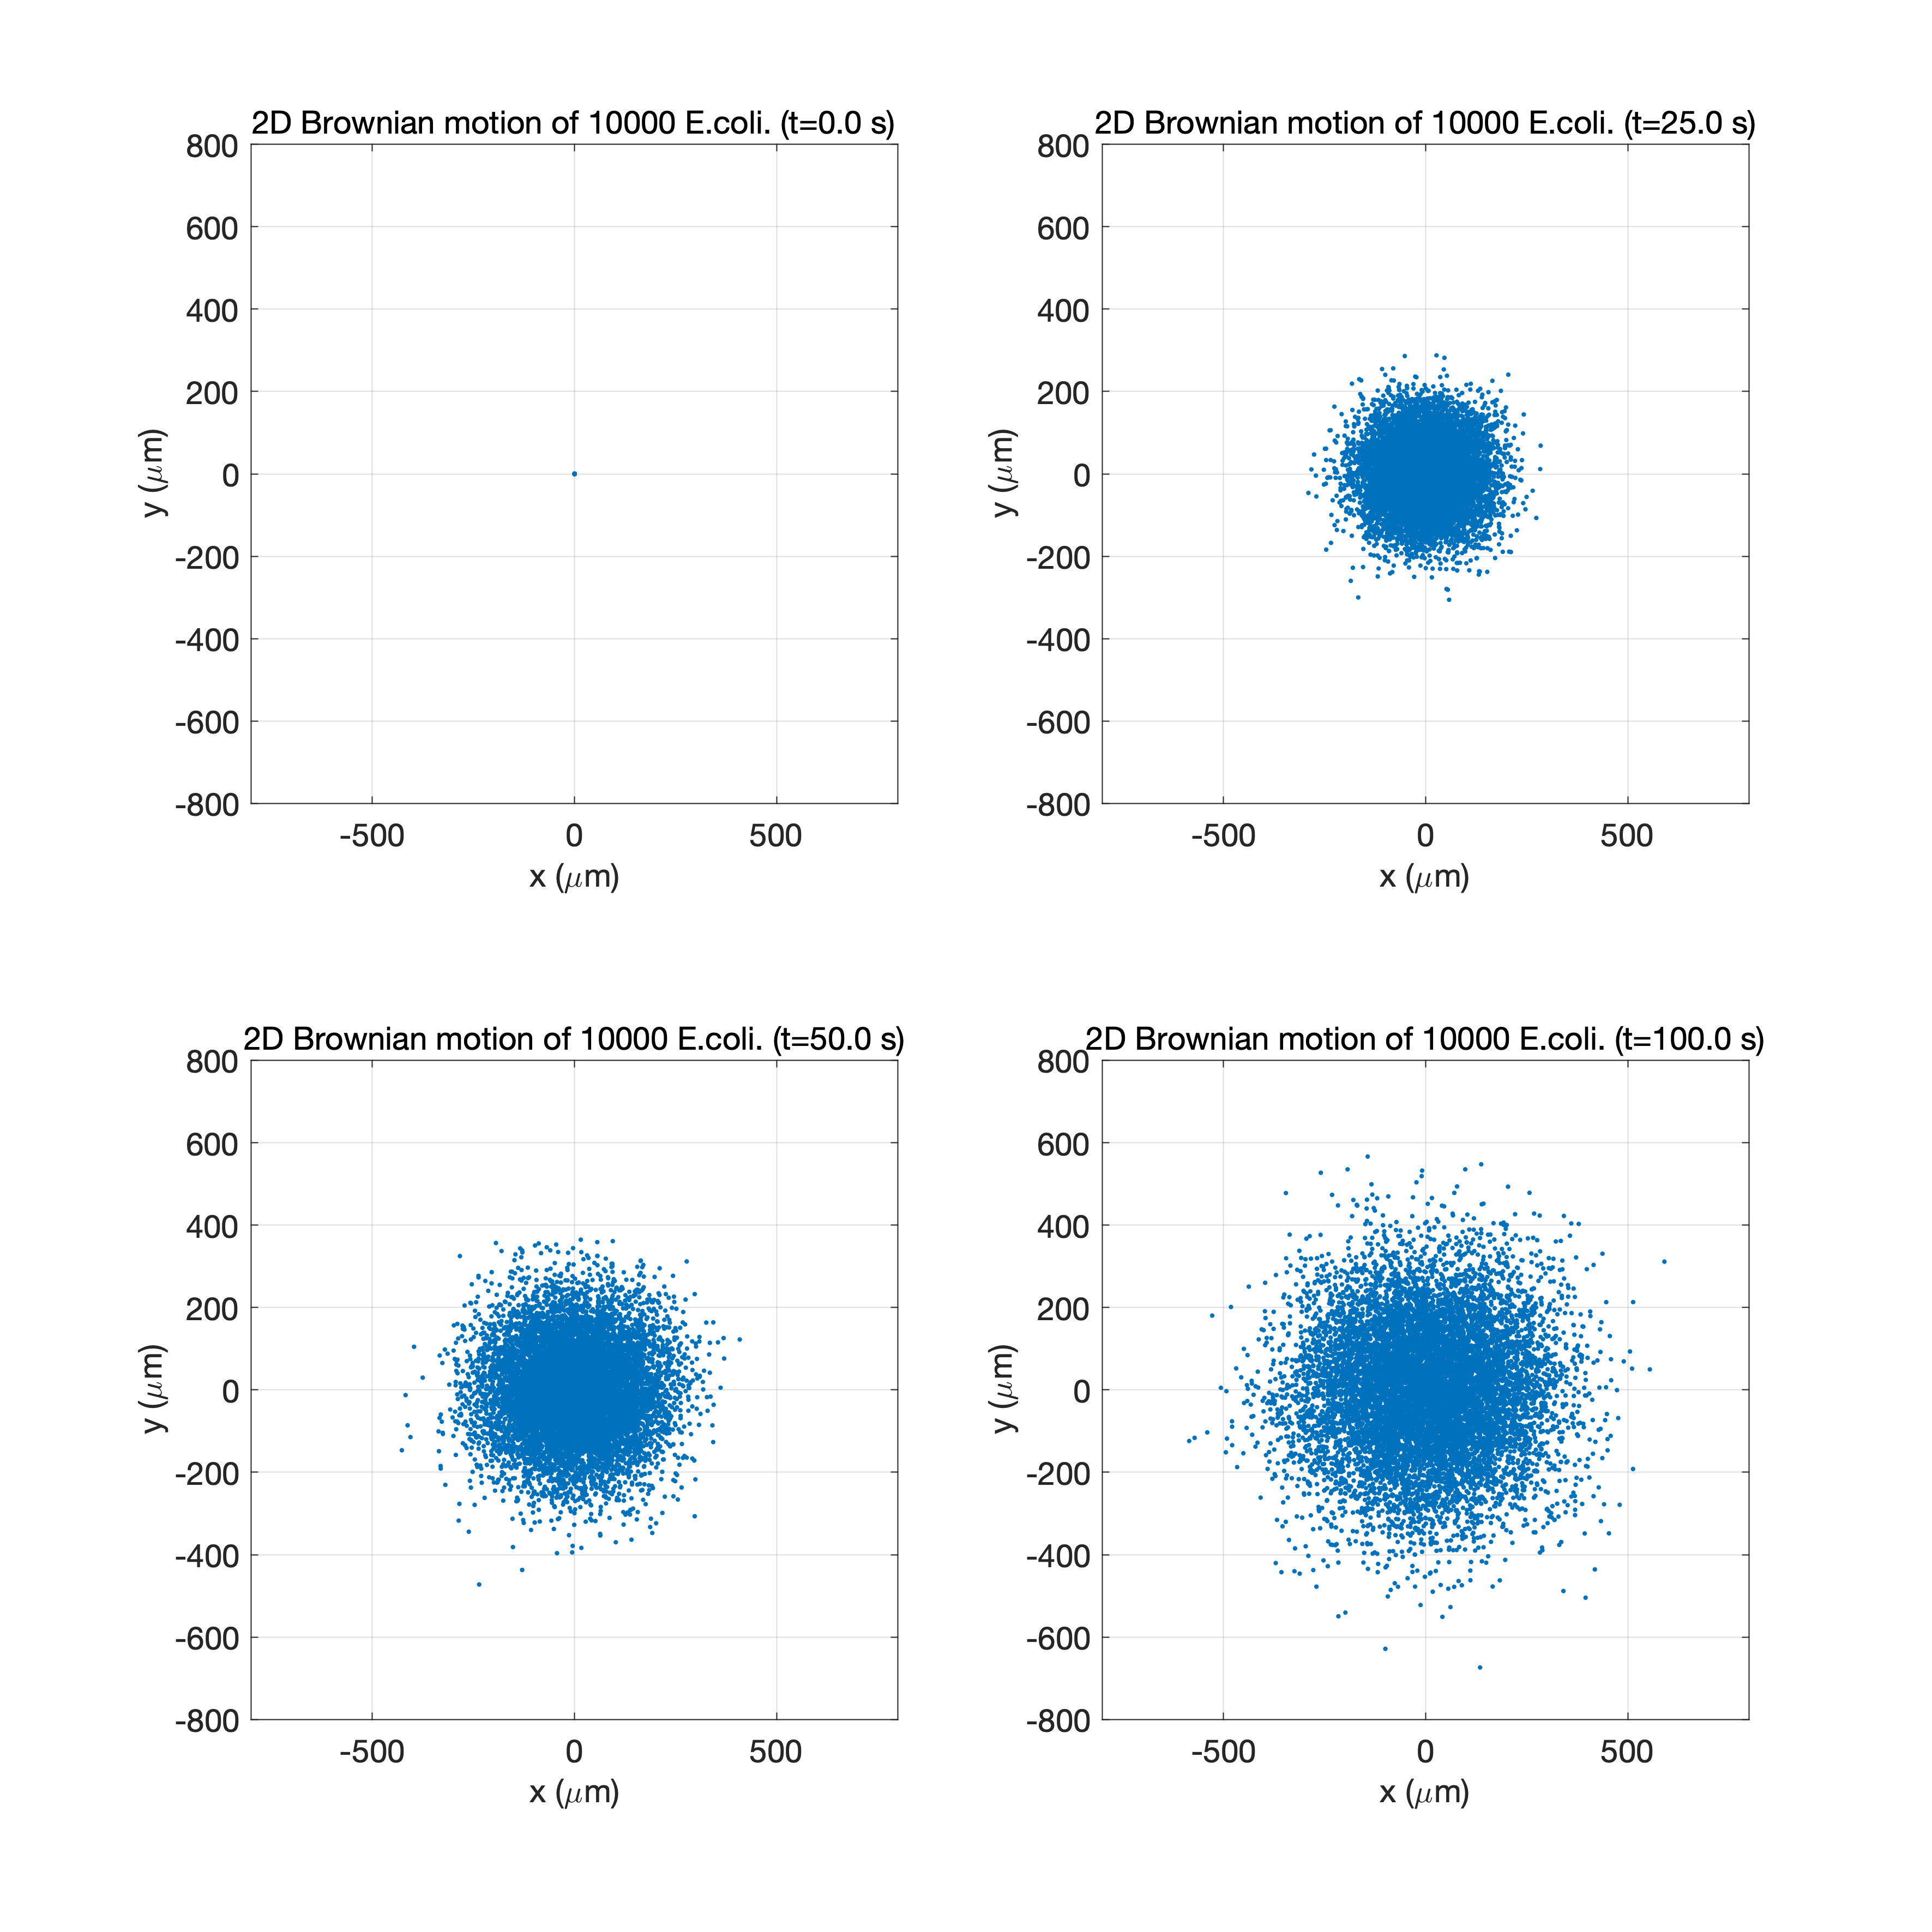
\includegraphics[width=1\linewidth]{Figures/P1_fig1.png}
\caption{The simulation of 10000 $E.coli$ cells for simple 2D Brownian motion form (0,0) after 100s}
\label{P1_fig1}
\end{figure}

\begin{figure}[H]
\centering
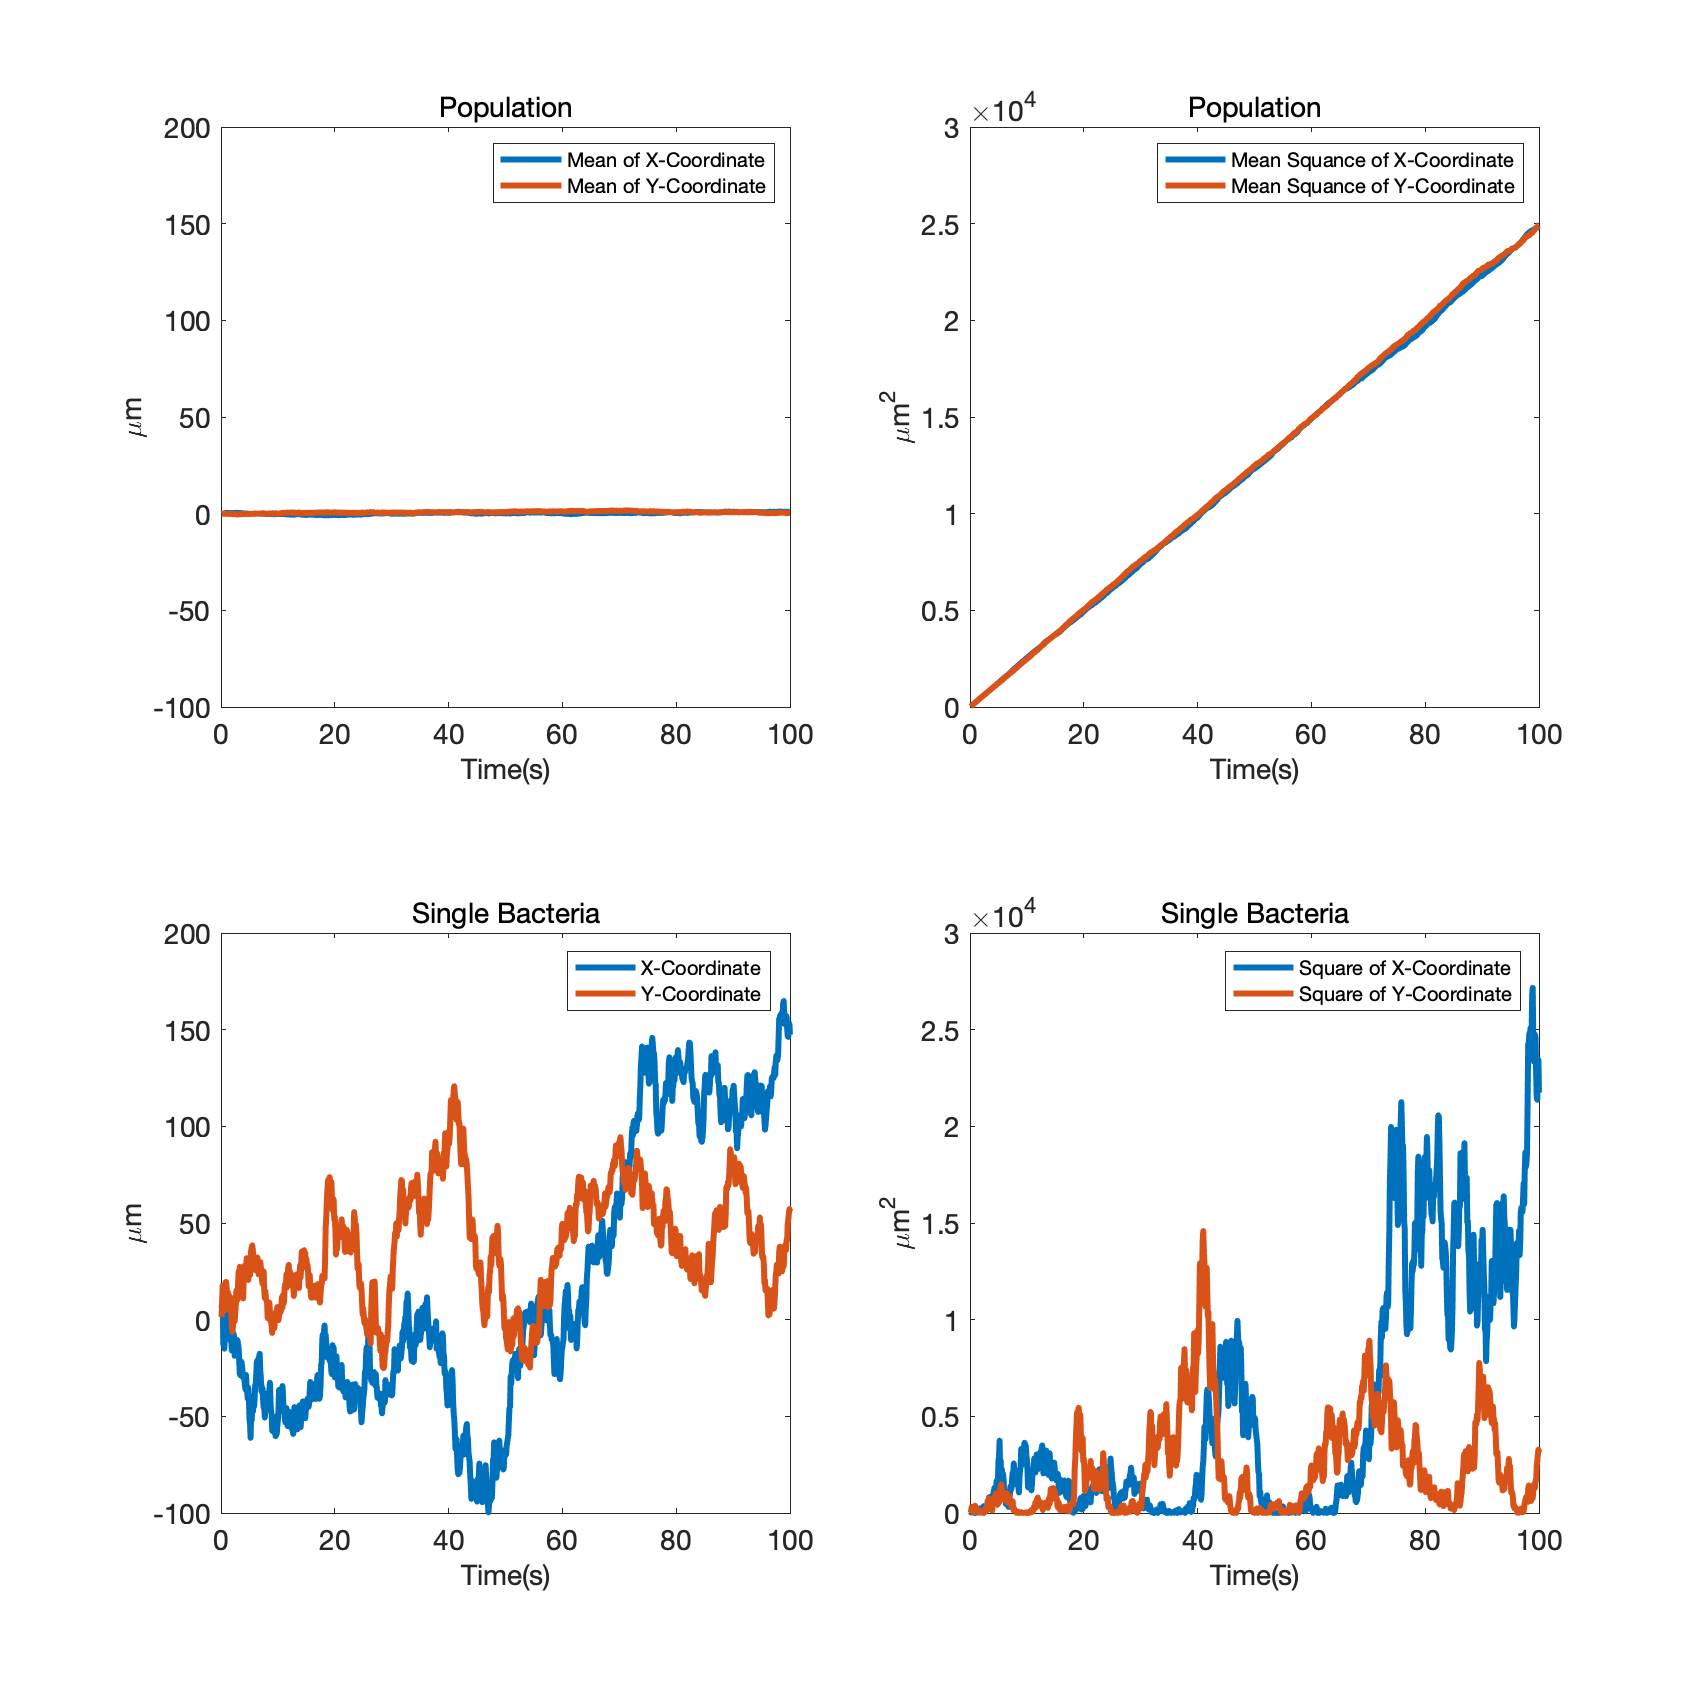
\includegraphics[width=1\linewidth]{Figures/P1_fig2.png}
\caption{The ”mean displacement” and ”mean displacement-square” overtime for simple 2D brownic motion}
\label{P1_fig2}
\end{figure}


\begin{figure}[H]
\centering
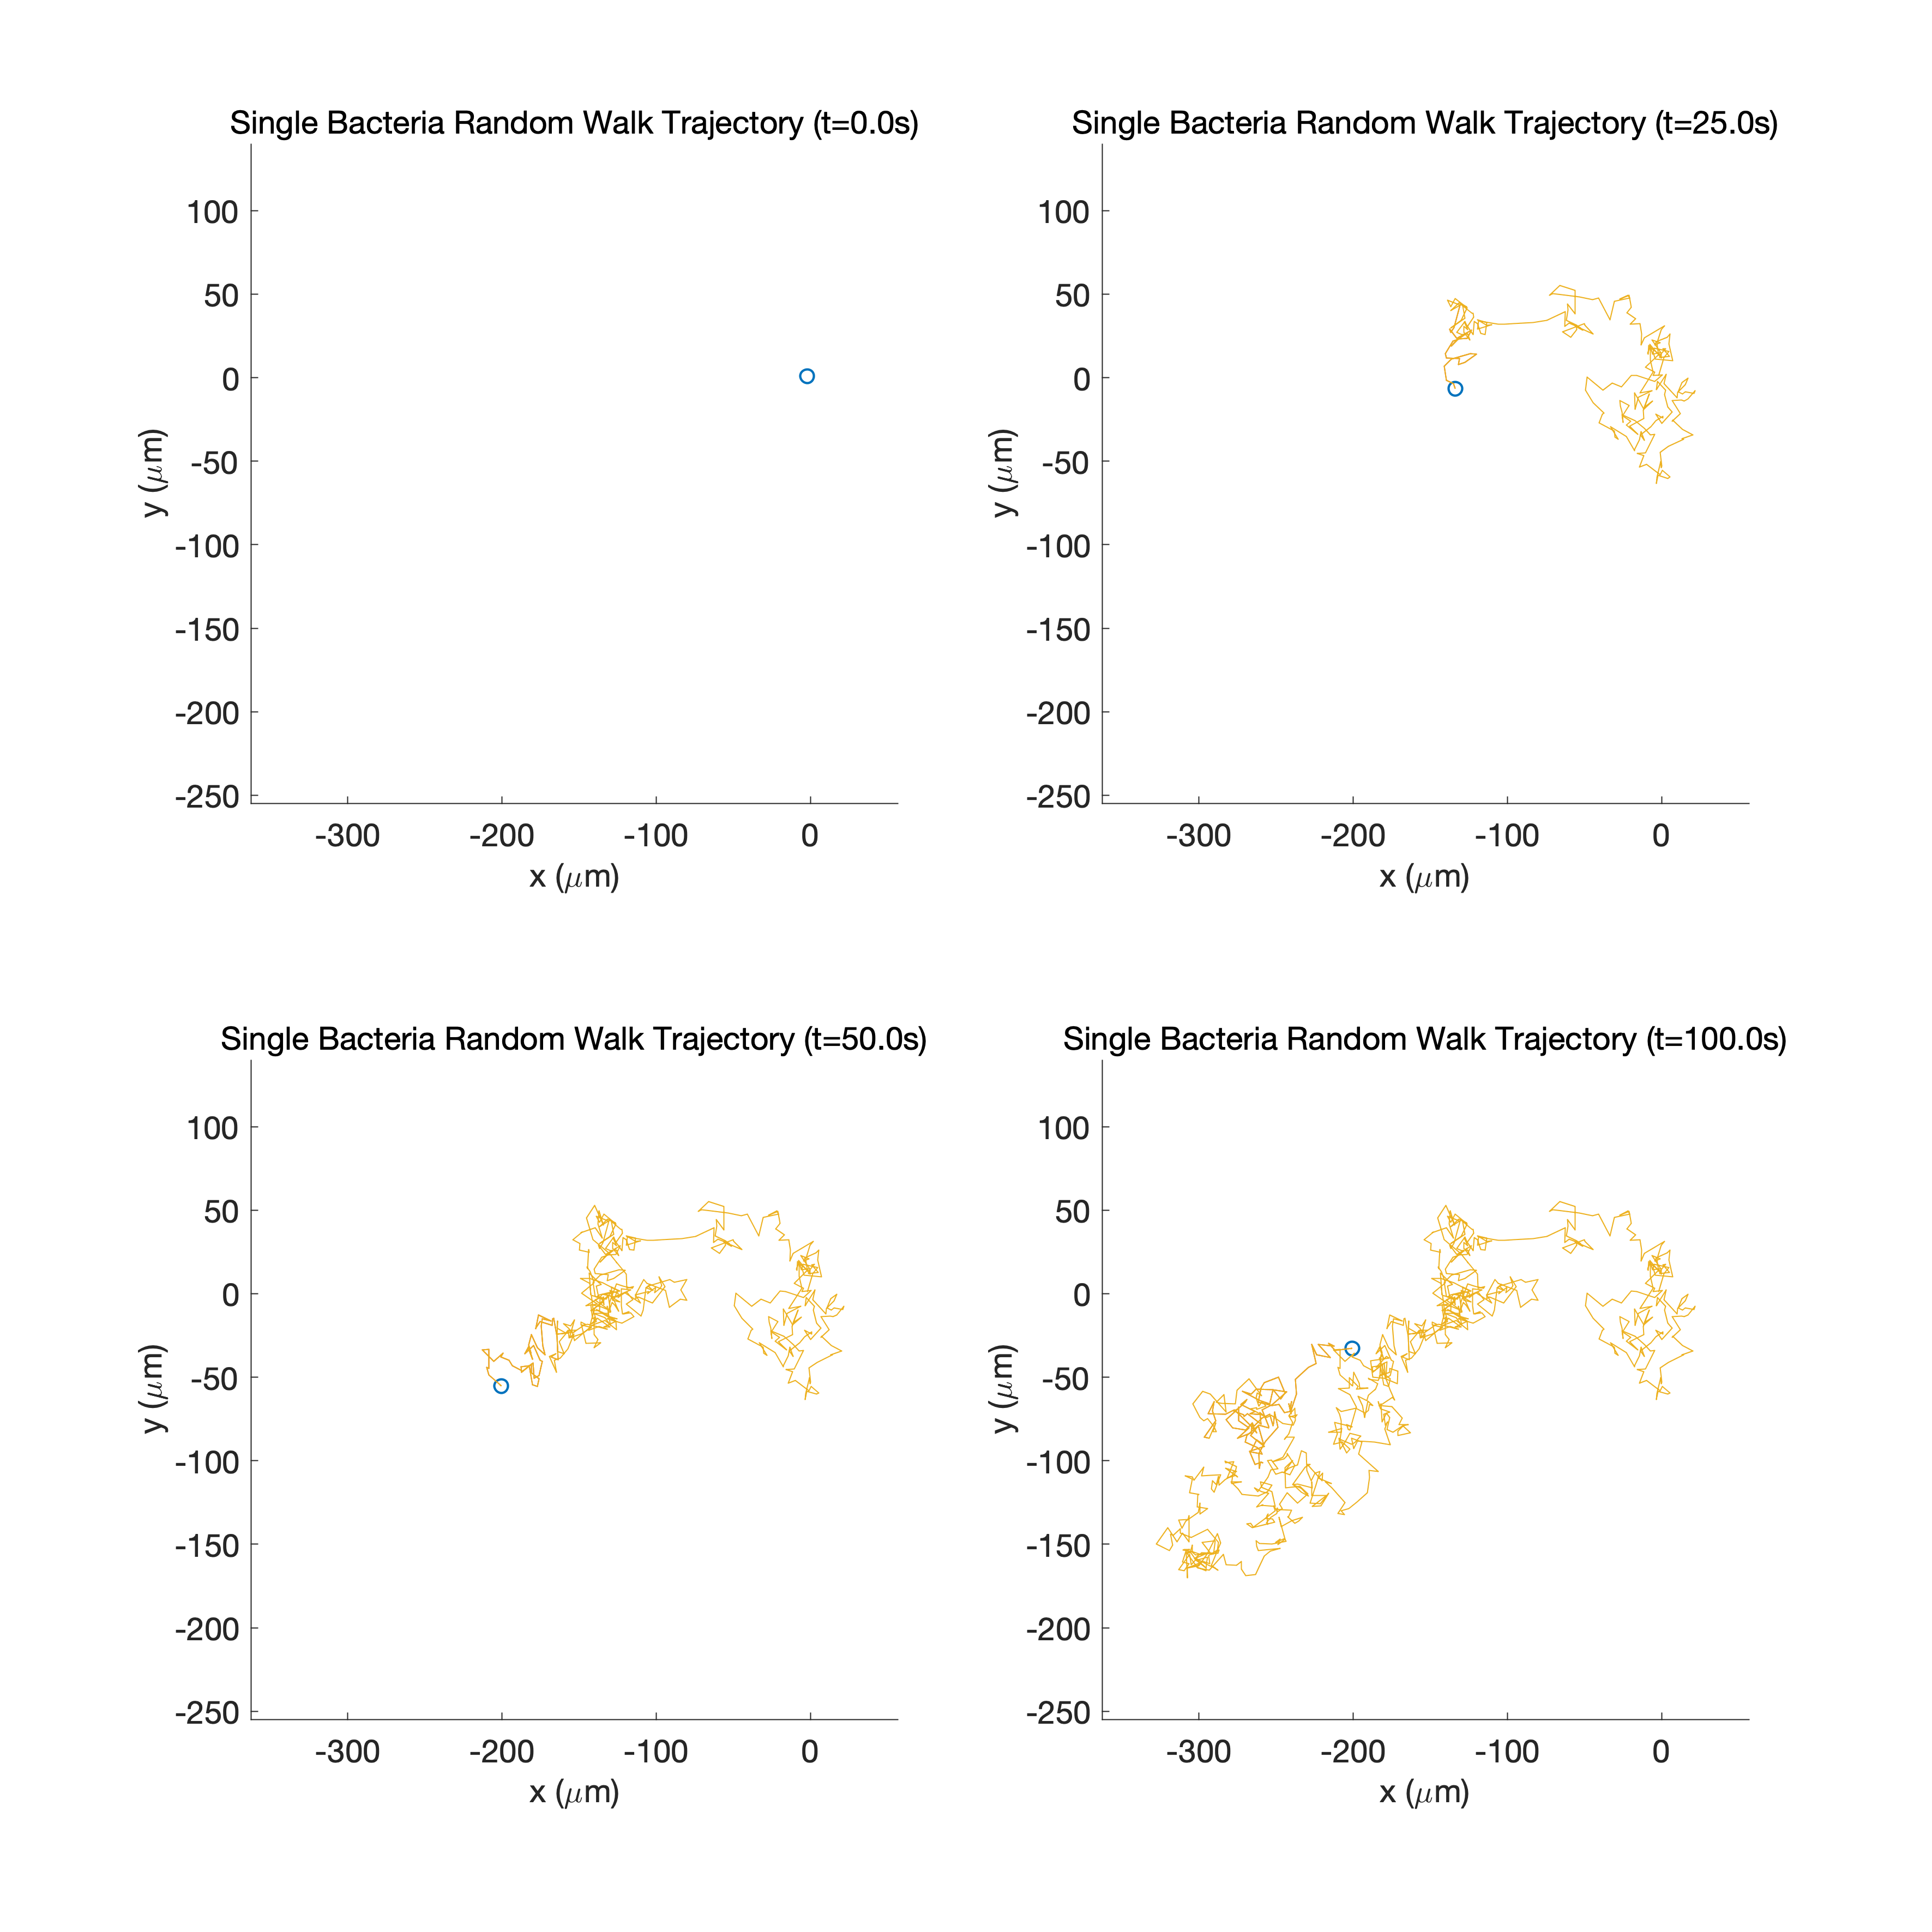
\includegraphics[width=1\linewidth]{Figures/P1_fig3.png}
\caption{Single Bacteria Random Walk Trajectory}
\label{P1_fig2}
\end{figure}


%----------------------------------------------------------------------------------------







%----------------------------------------------------------------------------------------



%----------------------------------------------------------------------------------------




%The \code{biblatex} package is used to format the bibliography and inserts references such as this one \parencite{Reference1}. The options used in the \file{main.tex} file mean that the in-text citations of references are formatted with the author(s) listed with the date of the publication. Multiple references are separated by semicolons (e.g. \parencite{Reference2, Reference1}) and references with more than three authors only show the first author with \emph{et al.} indicating there are more authors (e.g. \parencite{Reference3}). This is done automatically for you. To see how you use references, have a look at the \file{Chapter1.tex} source file. Many reference managers allow you to simply drag the reference into the document as you type.

